\documentclass[bibliography=totocnumbered,a4paper,10pt,oneside]{scrbook}
\usepackage[utf8]{inputenc}
\usepackage{amsmath,amsthm, amssymb, latexsym}
\usepackage{epstopdf,graphicx}
\usepackage[hidelinks]{hyperref}
\usepackage{listings,xcolor,float,multirow}
\usepackage{array}
\usepackage{longtable}

\usepackage[a4paper, total={6in, 9in}]{geometry}
\usepackage{xspace}

\usepackage{pdfpages}

%==============%
%  Code Style  %
%==============%
\definecolor{serenity-green}{rgb}{0.1875,0.46875,0.0}
\lstset{
  basicstyle=\ttfamily,
  commentstyle=\color{gray}\ttfamily,
  columns=fullflexible,
  language=bash,
  frame=l,
  showstringspaces=false,
  backgroundcolor = \color{serenity-green!30}
}



%==========%
%  Macros  %
%==========%

\newcommand{
\serenity}{\textsc{Serenity}\xspace}

\newcommand{\ttt}[1]{%
  \begingroup\setlength{\fboxsep}{1pt}%
  \colorbox{serenity-green!30}{\texttt{\hspace*{2pt}\vphantom{(g}#1\hspace*{2pt}}}%
  \endgroup
}

%==============%
%  References  %
%==============%
\usepackage[backend=bibtex,
            sorting=none,
            style=chem-angew]{biblatex}
\addbibresource{SerenityUserManual.bib}

%============%
%  Document  %
%============%
\begin{document}
\thispagestyle{empty}
\begin{center}
\vspace*{1cm}

\includegraphics[width=0.95\textwidth]{./figs/SerenityLogo.png}\\
%{\Huge
% \textsc{Serenity}
%}\\
\vspace{2cm}
{\LARGE\textbf{
User Manual
}}\\
\vspace{1cm}
{\large\textbf{
Program Version: 1.6.1\\
Manual Generated: \today
}}\\
\vspace{2cm}
{\large\textbf{
The Serenity Developers$^{\dagger}$\footnote{Release Repository: \texttt{http://github.com/qcserenity/serenity}}
\footnote{For questions and requests pertaining the manual please contact:\\ \texttt{serenity@uni-muenster.de}}
}}\\
\vspace{2cm}
{\large Manual layout by: \\
Jan P.\ Unsleber
}
\\[2ex]

$^{\dagger}$ Theoretische Organische Chemie,
Organisch-Chemisches Institut \\
and Center for Multiscale Theory and Computation,\\
Universit\"at M\"unster\\
Corrensstra{\ss}e 40, 48149 M\"unster, Germany\\[2ex]

\vfill
\end{center}
\newpage
\pagenumbering{Roman}
\setcounter{page}{1}
\tableofcontents

\newpage
\pagenumbering{arabic}
\setcounter{page}{1}
\numberwithin{equation}{subsection}

\input{misc/preface.tex}

% =============================
%   Installation Instructions
% =============================

\input{installation/install.tex}

% =================================
%   Text input: Systems and Tasks
% =================================

\input{input/textInput.tex}

% ==========
%   Python
% ==========

\clearpage
\input{python/python.tex}

\newpage

% ====================================
%   Bugs, Feedback, Feature Requests
% ====================================

\input{misc/feedback.tex}

% ========================
%   Theoretical Background
% ========================
\clearpage
\chapter{Theoretical Background}
\section{Pseudo-natural Orbital Construction}
The purpose of this section is to explain the pair natural orbital (PNO), triple-natural orbital (TNO) and
quasi canonical projected atomic orbital (QC-PAO) construction. We will refer to PNOs and TNOs as pseudo-natural
orbitals in the following section. We will always assume restricted Hartree-Fock orbitals as our reference orbitals.
This section is based on the following references~\cite{Pulay1983,Neese2009b,Riplinger2013a}.

\subsection{Redundant Projected-Atomic Orbital Construction}
In every local correlation method some sort of local representation of the virtual orbitals in necessary.
Since \textsc{Serenity} mainly implements Domain-based Local Pair Natural Orbital (DLPNO)-based correlation
methods, the virtual space is constructed from projected atomic orbitals (PAOs).
These PAOs $\{|\tilde{\mu}\rangle\}$ are given by
\begin{align}
  |\tilde{\mu}\rangle = \left(1-\sum_{i} |i\rangle\langle i|\right)|\mu\rangle,
  \label{eq:pao}
\end{align}
where the sum runs over all occupied orbitals $|i\rangle$.

These PAOs represent a virtual orbital set that fully spans the virtual orbital space, is linear dependent
and the functions are not necessarily normalized.
The coefficients $\pmb{C}^{\mathrm{PAO}}$ of the redundant, unnormalized PAOs are given in matrix
notation by
\begin{align}
  \pmb{C}^{\mathrm{PAO}} = \pmb{1}-\frac{1}{2} \pmb{D}\pmb{S}^\mathrm{AO},
\end{align}
where $\pmb{1}$ is the identity matrix, $\pmb{D}$ the density matrix in atomic orbital (AO) basis and
$\pmb{S}^\mathrm{AO}$ the overlap matrix in AO basis.

These PAOs are refined further by omitting functions which have a negligible norm
[e.g. $1$s basis functions may be fully removed by the projection in Eq.~(\ref{eq:pao})]
and normalizing all remaining functions.
We will refer to the resulting PAOs as redundant PAOs, since the linear dependencies within the function
sets are still present.

\subsection{Redundant Projected-Atomic Orbital Selection}
In order to motivate the truncation of the PAO space for a specific orbital, orbital pair or orbital triple,
we consider the M{\o}ller--Plesset perturbation theory (MP2) pair energy $\epsilon_{ij}^\mathrm{MP2}$ for
a given pair $ij$. This energy is given by~\cite{Pulay1983}
\begin{align}
  \epsilon_{ij}^\mathrm{MP2} = \frac{1}{1+\delta_{ij}}\sum_{ab}{(ia|jb)}(4t^{ij}_{ab}-2t^{ij}_{ba}),
  \label{eq:MP2PairEnergy}
\end{align}
where the two electron exchange integral $(ia|jb)$ is given in $(11|22)$ notation, referring to the integration
variables. The $t^{ij}_{ab}$ are the MP2 amplitudes. The virtual functions are denoted by $a$ and $b$.
The only restriction for the choice in virtual functions is that they are orthogonal to the occupied orbital set.
It is obvious from Eq.~(\ref{eq:MP2PairEnergy}) that terms in the sum can only contribute, if $i$ and $a$ as well as $j$
and $b$ have non-zero differential overlap. Thus, PAOs are assigned to occupied orbitals $i\rightarrow [i]$.
We call $[i]$ the PAO domain of $i$. The PAO domains of an orbital pair $[ij]$ are constructed
as the union of the PAO domains of the individual orbitals $[ij]=[i]\cup [j]$. The same is done for orbital
triples ($[ijk]=[i]\cup [j]\cup [k]$).

\subsection{Quasi-Canonical Projected-Atomic Orbital Construction}
Within the truncated, redundant PAO sets, the PAOs are orthogonalized by constructing the PAO--PAO overlap matrix
in the PAO domain and diagonalizing it. The resulting eigenvectors of the PAO--PAO overlap matrix are
truncated by eigenvalue in order to remove (nearly) linear dependent vectors.

Then the Fock matrix is transformed into the basis of these non-redundant PAOs and diagonalized. The resulting functions
are now called quasi-canonical PAOs (QC-PAOs). This quasi-canonicalization is extremely convenient for local
second order M{\o}ller--Plesset perturbation theory (MP2), since the iterative amplitude optimization proofed
to converge exceptionally well. Furthermore, the QC-PAOs are needed to calculate semi-canonical MP2 (SC-MP2)
amplitudes which will become important in the next step.

\subsection{Pseudo Natural Orbital Construction}

The QC-PAO sets which are necessary to get reasonable accurate results are often very large. Thus, the size of the
virtual orbital space is reduced further by constructing pseudo natural orbitals. For orbital pairs, we can easily
motivate this by reconsidering Eq.~(\ref{eq:MP2PairEnergy}), which we already used in order to reduce the size of
the initial redundant PAO sets. The idea is to find a reasonable approximation to the MP2 amplitudes $\pmb{t}_{ij}$
and then use this information to find a basis in which the sum in Eq.~(\ref{eq:MP2PairEnergy}) becomes very
compact~\cite{Neese2009b}.

As an approximation to the MP2 amplitudes SC-MP2 amplitudes are used. The latter are given by
\begin{align}
  t^{ij}_{\tilde{\mu},\tilde{\nu}} &= -\frac{(i\tilde{\mu}|j\tilde{\nu})}{{\epsilon_{\tilde{\mu}}}+{\epsilon_{\tilde{\nu}}}-F_{ii}-F_{jj}},
\end{align}
where $\epsilon_{\tilde{\mu}}$ and $\epsilon_{\tilde{\nu}}$ are the eigenvalues of the QC-PAOs and $F_{ii}$ and $F_{jj}$
are diagonal Fock matrix elements.
From these amplitudes natural orbitals are constructed by diagonalizing the pair density matrix $\pmb{D}^{ij}$ given
by
\begin{align}
  \mathbf{D}^{ij} &= \tilde{\mathbf{t}}^{ij}\mathbf{t}^{ij\dagger} + \tilde{\mathbf{t}}^{ij\dagger}\mathbf{t}^{ij},
\end{align}
where $\tilde{t}^{ij}_{\tilde{\mu},\tilde{\nu}}$ is given by
\begin{align}
  \tilde{t}^{ij}_{\tilde{\mu},\tilde{\nu}}  &= \frac{1}{1+\delta_{ij}}(4t^{ij}_{\tilde{\mu}\tilde{\nu}}-2t^{ij}_{\tilde{\nu}\tilde{\mu}}).
\end{align}

The eigenvectors of $\mathbf{D}^{ij}$ are truncated by their eigenvalues and the remaining functions are
rotated such that they diagonalize the Fock matrix.

The pseudo-natural orbitals for singles of orbital $i$ are constructed from the PNOs of the
diagonal pair $ii$ by adjusting the truncation threshold for the PNOs.

For orbital triples, a triple-density matrix $\mathbf{D}^{ijk}$ is constructed from the pair density matrices
of the orbital pairs~\cite{Riplinger2013a} $ij$, $ik$ and $jk$ as
\begin{align}
  \mathbf{D}^{ijk} = \frac{1}{3} \left( \mathbf{D}^{ij} + \mathbf{D}^{ik} +\mathbf{D}^{jk} \right).
\end{align}
The remaining procedure for the Triple-natural Orbital (TNO) construction is the same as for the PNOs.
However, in case of a triples correction to the correlation energy, the converged amplitudes of the orbital
pairs are usually used for the TNO construction instead of the SC-MP2 guess.

\section{Domain-Based Local Pair Natural Orbital Coupled Cluster Equations}
This text should document the implementation of Domain Localized Pair Natural Orbital (DLPNO) Coupled Cluster
containing single and double substitutions (DLPNO-CCSD) with semi-canonical triple correction [DLPNO-CCSD(T$_0$)]
in \textsc{Serenity}. This implementation was first presented in Ref.~(\cite{Bensberg2020}).

DLPNO-CCSD is an approximation to the full canonical CCSD. However, since the PNOs used as a local virtual
space will constitute the full set of canonical virtual orbitals, if all truncation thresholds approach zero,
DLPNO-CCSD has to approach the canonical coupled cluster results in this limit (Note that approximations to
the two electron integrals may influence the results on a different level).
The same is only given for DLPNO-CCSD(T$_0$) if canonical occupied orbitals are used.
If the orbitals are localized the triples correction may deviate.

\subsection{DLPNO-CCSD Equations}
The main task of the CCSD and the DLPNO-CCSD procedure is to calculate the coupled cluster amplitudes.
This is done in an iterative procedure since the equations for the amplitudes are coupled.

In the following, $i,j,k...$ will refer to internal orbitals, $a,b,c...$ to external orbitals, $\pmb{t}^i$
are the single amplitudes of orbital $i$, and $\pmb{t}^{ij}$ the double amplitudes of pair $ij$. As usual,
the Fock matrix is denoted by $\pmb{F}$, the exchange operator in matrix representation by
${K}^{ij}_{ab}=(ia|jb)$, and the coulomb matrix by $J^{ij}_{ab}=(ij|ab)$. All integrals are given in $(11|22)$
notation, where the indices $1$ and $2$ refer to the integration variables.

The singles residual $R_{a}^{i}$ equations for substitution of the internal orbital $i$ with the external orbital
$a$ are given by
\begin{align}
  \begin{split}
    R_{a}^{i}  &= F_{ia}+\left(\pmb{\tilde{F}}^\dagger \pmb{t}^i\right)_a+G(\pmb{t_1})_{ia}-\sum_j \tilde{F}_{ij}t^j_a\\
               & +\sum_{j} \left[(2\pmb{t}^{ij}-\pmb{t}^{ij\dagger})\pmb{\tilde{F}}_{j}\right]_a-\sum_{kjb} \tau_{ab}^{kj} \left(2(ik|jb)-(ij|kb)\right)\\
               & +{\sum_{jbc}(jc|ab)(2\pmb{\tau}^{ij}-\pmb{\tau}^{ji})_{bc}}\\
               & +\sum_{jb}\left(\tilde{F}_{jb}-2F_{jb}\right)t^i_bt^j_a,
  \end{split}
\end{align}
and the equations for the doubles residuals $R^{ij}_{ab}$ are given by
\begin{align}
  \begin{split}
    R^{ij}_{ab} &= K_{ab}^{ij} + K(\pmb{\tau}_{ij})_{ab}
                + (\pmb{\tilde{\tilde{F}}}^\dagger{\pmb{t}^{ij}}+{\pmb{t}^{ij}}\pmb{\tilde{\tilde{F}}})_{ab}
                -\sum_k (\tilde{\tilde{F}}_{jk}\pmb{t}^{ki\dagger}+\tilde{\tilde{F}}_{ik}\pmb{t}^{kj})_{ab}
                \\&+\sum_{kl}\widetilde{(ik|jl)}\tau_{ab}^{kl}\\
                &+{\sum_k \left[ (2\pmb{t}^{ki\dagger}-\pmb{t}^{ki}) \pmb{\tilde{K}}^{kj}+\pmb{\tilde{K}}^{ki\dagger}(2\pmb{t}^{kj}-\pmb{t}^{kj\dagger})\right]_{ab}}\\
                &{-\sum_k \left(\frac{1}{2}\left[\pmb{t}^{ki}\pmb{J}^{kj}+\pmb{J}^{ki\dagger}\pmb{t}^{kj\dagger}\right]
                +\pmb{t}^{kj} \pmb{J}^{ki} + \pmb{J}^{kj\dagger}\pmb{t}^{ki\dagger}\right)_{ab}}\\
                &{ - \sum_k \left((jk|ia)t_b^k + (ik|jb)t_a^k \right) + {\sum_c (jb|ac)t_c^i + (ia|bc)t_c^j}}\\
                &- \sum_k \left( \left(\pmb{K}^{ik}\pmb{t}^j\right)_at_b^k + \left(\pmb{K}^{jk}\pmb{t}^i\right)_b t_a^k
                + \left(\pmb{J}^{ik}\pmb{t}^j\right)_b t_a^k + \left(\pmb{J}^{jk}\pmb{t}^i\right)_a t_b^k \right).
  \end{split}
\end{align}

The ``dressed'' integrals and intermediates are given by
\begin{align}
  \pmb{\tau}^{ij} = \pmb{t}^{ij}+\pmb{t}^i\pmb{t}^{j\dagger},
\end{align}
\begin{align}
  \tilde{F}_{ij} = F_{ij} + \sum_k \left\langle {(2\pmb{K}^{jk\dagger}-\pmb{K}^{jk})}\pmb{\tau}^{ik}\right\rangle,
\end{align}
\begin{align}
  \pmb{\tilde{F}} = \pmb{F} - {\sum_{kl}\left(2\pmb{K}^{kl}-\pmb{K}^{kl\dagger}\right)\pmb{\tau}^{lk}},
\end{align}
\begin{align}
  \pmb{\tilde{F}}_i = \pmb{F}_i + \sum_k\left(2\pmb{K}^{ik}-\pmb{K}^{ik\dagger}\right)\pmb{t}^k,
\end{align}
\begin{align}
  \tilde{\tilde{F}}_{ij} = \tilde{F}_{ij} + G(\pmb{t_1})_{ij} + {\pmb{F}_j^\dagger \pmb{t}^i},
\end{align}
\begin{align}
  \pmb{\tilde{\tilde{F}}} = \pmb{\tilde{F}} + \pmb{G(t_1)}-\sum_i{\pmb{F}_i \pmb{t}^{i\dagger}},
\end{align}
\begin{align}
  G(\pmb{t_1})_{pq} = \sum_{jb} t_b^j \left[2(pq|jb)-(pj|qb)\right],
\end{align}
\begin{align}
  K(\pmb{\tau^{ij}})_{ab} = \sum_{cd} \left((ac|bd) - \sum_k (kd|ac)t_b^k+(kc|bd)t^k_a \right)\tau^{ij}_{cd},
\end{align}
\begin{align}
  \widetilde{(ik|jl)} = (ik|jl) + \left\langle \pmb{\tau}^{ij}\pmb{K}^{lk}\right\rangle+\sum_a (ki|la)t_a^j+(lj|ka)t_a^i,
\end{align}
\begin{align}
  \begin{split}
    \tilde{K}^{ij}_{ab} &=
                         K^{ij}_{ab} + \sum_c (ia|bc)t_c^j-\frac{1}{2}\left(J^{ij}_{ab}+\sum_c(ab|ic)t_c^j\right)\\
                        &+\sum_k \frac{1}{4}\left[(2\pmb{K}^{ik}-\pmb{K}^{ik\dagger})(2\pmb{t}^{kj}-\pmb{t}^{kj\dagger})\right]_{ab}\\
                        &-\frac{1}{2}\left[ 2(ia|kj)-(ak|ij) \right]t^k_b+\left[ (2\pmb{K}^{ik}-\pmb{K}^{ik\dagger})\pmb{t}^j\pmb{t}^{k\dagger} \right]_{ab}
  \end{split}
\end{align}
and
\begin{align}
  \tilde{J}^{ij}_{ab}=J^{ij}_{ab}+\sum_c (ab|ic)t^j_c-\sum_k \frac{1}{2}\left( \pmb{K}^{ki}\pmb{t}^{jk}\right)_{ab}+(ak|ij)t^k_b+\left(\pmb{K}^{ki}\pmb{t}^j\pmb{t}^{k\dagger}\right)_{ab}.
\end{align}
The operator $\langle~\rangle$ is evaluated as
\begin{align}
  \langle\pmb{AB}\rangle = \sum_{ab} A_{ab} B_{ba}.
\end{align}

Note that the sigma vector $G(\pmb{t_1})_{pq}$ can be written in atomic orbital basis in a Fock-matrix-like fashion
as
\begin{align}
  \begin{split}
    G(\pmb{t_1})_{pq} &= \sum_{jb} t_b^j \left[2(pq|jb)-(pj|qb)\right]\\
                      &= \sum_{jb} t_b^j \sum_{\mu\nu} c_{\mu j} c_{\nu b} \left[ 2(pq|\mu\nu)-(p\mu|q\nu) \right]\\
                      &= \sum_{\mu\nu} \underbrace{\sum_{jb} t_b^j c_{\mu j} c_{\nu b}}_{d_{\mu\nu}}
                         \left[ 2(pq|\mu\nu)-(p\mu|q\nu) \right]\\
                      &= \sum_{\mu\nu} d_{\mu\nu} \left[ 2(pq|\mu\nu)-(p\mu|q\nu) \right].
  \end{split}
  \label{eq:SigmaVectorAO}
\end{align}
Thus, it can be evaluated in the same way as sigma vectors in response calculations before transforming them to
the molecular orbital basis. The sigma vector $G(\pmb{t_1})_{pq}$ is constructed as a matrix and transformed on
the fly to the necessary basis ($G(\pmb{t_1})_{ij}$, $G(\pmb{t_1})_{ia}$ and $G(\pmb{t_1})_{ab}$).

\subsection{Semi-Canonical Triples Correction}
In the DLPNO-CCSD(T$_0$)~\cite{Riplinger2013a} approach, the contribution of the triples
to the correlation energy is approximated in a semi-canonical fashion. This means that the same equations
are used which would be valid for canonical orbitals. Note that this is, of course, not necessarily correct for
local-coupled cluster. The triples correction is given by the equation of Rendell
\emph{et al.}~\cite{Rendell1991}\ as
\begin{align}
  \begin{split}
    \Delta E^{(T)} = \sum_{i\leq j\leq k} P_{ijk} \sum_{a\leq b\leq c }&
      \left[ (Y_{abc}^{ijk}-2Z_{abc}^{ijk})(W_{abc}^{ijk}+W_{bca}^{ijk}+W_{cab}^{ijk}) \right. \\
     &+ (Z_{abc}^{ijk}-2Y_{abc}^{ijk})({W_{acb}^{ijk}}+W_{bac}^{ijk}+W_{cba}^{ijk}) \\
     &+ \left. 3X_{abc}^{ijk}\right]
     /(\varepsilon_i+\varepsilon_j+\varepsilon_k-\varepsilon_a-\varepsilon_b-\varepsilon_c).
  \end{split}
\end{align}

The intermediates $V$, $W$, $X$, $Y$, and $Z$ are given by
\begin{align}
  \begin{split}
    W_{abc}^{ijk} &= \hat{P}^{abc}_{ijk} \left[ \sum_d t^{kj}_{cd}(ia|bd) -\sum_l t_{ab}^{il}(kc|jl) \right],\\
    V_{abc}^{ijk} &= \left(W_{abc}^{ijk}+t_a^i K^{jk}_{bc} + t_b^j K_{ac}^{ik}+t_c^k K_{ab}^{ij} \right)/P_{abc}\\
    X_{abc}^{ijk} &= W_{abc}^{ijk}V_{abc}^{ijk}+W_{acb}^{ijk}V_{acb}^{ijk}+W_{bac}^{ijk}V_{bac}^{ijk}
                   +W_{bca}^{ijk}V_{bca}^{ijk}\\
                  &+W_{cab}^{ijk}V_{cab}^{ijk}+W_{cba}^{ijk}V_{cba}^{ijk} \\
    Y_{abc}^{ijk} &= V_{abc}^{ijk}+V_{bca}^{ijk}+V_{cab}^{ijk}\\
    Z_{abc}^{ijk} &= V_{acb}^{ijk}+V_{bac}^{ijk}+V_{cba}^{ijk},
  \end{split}
\end{align}
and the permutation operators/factors by
\begin{align}
  \begin{split}
    P_{abc} &= 1+\delta_{ab}+\delta_{bc}\\
    P_{ijk} &= 2-\delta_{ij}-\delta_{jk}\\
    \hat{P}^{abc}_{ijk} {abc\choose ijk} &= {abc\choose ijk}+{acb\choose ikj}+{cab\choose kij}+{cba\choose kji}\\
                                         &+ {bca\choose jki}+{bac\choose jik}.
  \end{split}
\end{align}
The operator $\hat{P}^{abc}_{ijk}$ has to be understood as acting on a rank-six tensor with distinct indices $abc$
and $ijk$ and producing the sum of the permutations within these index sets, as shown above.

In local coupled cluster, the eigenvalues $\varepsilon_a$, which correspond to virtual functions, are substituted
by the (pseudo) eigenvalues of the triple-natural orbitals of the triple $ijk$, and the eigenvalues
corresponding to occupied orbitals $\varepsilon_i$ are substituted by the diagonal Fock-matrix elements
$F_{ii}$ (and $F_{jj}$ and $F_{kk}$).

The energy-correction increment for each triple $ijk$ can be calculated independently from all other triples, thus
allowing for easy and efficient parallelization of the calculation.

\section{Orbital Alignment Strategies}
\label{sec:OrbitalAlignmentStrategies}
This text documents the orbital alignment strategies available in \textsc{Serenity}. They were
first published in Ref.~(\cite{Bensberg2020}).

The task at hand is to align a set of orbitals $\{|i_L\rangle \}$ to a set of template orbitals
$\{|i_K\rangle\}$. We assume that both sets are of the same size and that each orbital in both
sets correspond to a point in the same partial charge space.
To put this into a simpler phrasing: Each orbital can be characterized by a set of orbital-wise partial charges for
which the charge centers (atoms, atom shells ...) are identical for both orbital sets. These partial charges will be
denoted as $ \{q_{iK}^a\} $ for orbital $|i_K\rangle$ and charge center $a$.

In order to arrive at a scheme that allows us to find a unitary transformation within the orbital set
$\{|i_L\rangle \}$ such that it becomes aligned to the template orbital set, we construct a penalty
function $S_{i}^P$ for each orbital as the difference between the partial charges to the power of an even exponent
$P$.
\begin{align}
  S_i^P = \sum_a(q_{iK}^a - q_{iL}^a)^P.
  \label{eq:similarityMeasure}
\end{align}
As partial charges we use shell-wise Intrinsic Atomic Orbital (IAO) charges~\cite{Knizia2013}, which are given by
\begin{align}
  q_{iL}^a = \langle i_L|\hat{n}_a|i_L\rangle
  \label{eq:IAOCharges}
\end{align}
where $\hat{n}_a$ is the projector on the functions of a shell $a$ of an orthonormal minimal-basis set for the
molecule
\begin{align}
   \hat{n}_a = \sum_{\rho\in a} |\rho\rangle\langle \rho |.
\end{align}
Note that the criterion can be adjusted freely. Partial charges work, but it is possible to
extend the list of criteria (e.g. by the orbital kinetic energy as discussed below).

Analogous to the IAO charges in Eq.~\ref{eq:IAOCharges}, cross charges can be defined as
\begin{align}
  q_{ijL}^a = \langle i_L|\hat{n}_a|j_L\rangle.
  \label{eq:IAOCrossCharges}
\end{align}

We can minimize the total penalty function $\sum_i S_i^P$ by iterative two by two rotations for all orbital pairs
within the set $\{|i_L\rangle \}$ with the constraint that the orbitals stay orthonormal.
This leads to a Lagrangian $L_\mathrm{rot}$ given for two rotated orbitals $|i^{\prime}_L\rangle$
and $|j^{\prime}_L\rangle$ as
\begin{align}
  \begin{split}
    L_\mathrm{rot}&=\sum_a^\mathrm{shells}\left[
      \left(q_{iK}^a-\langle i^{\prime}_L|\hat{n}_a|i_L^{\prime}\rangle \right)^P
    + \left(q_{jK}^a-\langle j^{\prime}_L|\hat{n}_a|j_L^{\prime}\rangle\right)^P
    \right]\\
    |i_L^{\prime}\rangle &= |i_L^{}\rangle \cos(\phi)+|j_L^{}\rangle\sin(\phi)\\
    |j_L^{\prime}\rangle &= |j_L^{}\rangle \cos(\phi)-|i_L^{}\rangle\sin(\phi).\\
  \end{split}
  \label{eq:LagrangianI}
\end{align}
Here, $|i_L\rangle$ and $|j_L\rangle$ are the initial, none-rotated orbitals.

Note that the orthonormality constrain is automatically fulfilled in Eq.~\ref{eq:LagrangianI} by
the definition of the rotated orbitals.

In the following we want to derive the working equations by inserting the definitions for $|i_L^{\prime}\rangle$
and $|j_L^{\prime}\rangle$ into $L_\mathrm{rot}$:
\begin{align}
  \begin{split}
    L_\mathrm{rot} &= \sum_a^\mathrm{shells}\left[
        \left(\underbrace{q_{iiK}^a-\cos^2(\phi)q_{iiL}^a-\sin^2(\phi)q_{jjL}^a-2\cos(\phi)\sin(\phi)q_{ijL}^a}
        _{L_\mathrm{rot}^{ia}}\right)^P\right.\\
        &~~~~~~~+\left.
        \left(\underbrace{q_{jjK}^a-\cos^2(\phi)q_{jjL}^a-\sin^2(\phi)q_{iiL}^a+2\cos(\phi)\sin(\phi)q_{ijL}^a}
        _{L_\mathrm{rot}^{ja}}\right)^P\right]\\
                   &=\sum_a^\mathrm{shells}\left[
                   \left(L_\mathrm{rot}^{ia}\right)^P+ \left(L_\mathrm{rot}^{ja}\right)^P
                   \right]
  \end{split}
\end{align}
With the elements of the sum $L_\mathrm{rot}^{ia}$ and $L_\mathrm{rot}^{ja}$ we can write the derivative of
$L_\mathrm{rot}$ with respect to the angle $\phi$ as
\begin{align}
  \frac{\partial L_\mathrm{rot} }{\partial \phi} &= \sum_a P \left[
        \left(L_\mathrm{rot}^{ia}\right)^{P-1} \frac{\partial L_\mathrm{rot}^{ia}}{\partial \phi}+
        \left(L_\mathrm{rot}^{ja}\right)^{P-1} \frac{\partial L_\mathrm{rot}^{ja}}{\partial \phi}
                                                   \right]
\end{align}
with
\begin{align}
  \frac{\partial L_\mathrm{rot}^{ia}}{\partial \phi} = 2\cos(\phi)\sin(\phi)(q_{iiL}^a-q_{jjL}^a)
                                                     +2[\sin^2(\phi)-\cos^2(\phi)]q_{ijL}^a
\end{align}
and find
\begin{align}
  \begin{split}
    \frac{\partial L_\mathrm{rot}^{ja}}{\partial \phi} &= -2\cos(\phi)\sin(\phi)(q_{iiL}^a-q_{jjL}^a)
                                                         -2[\sin^2(\phi)-\cos^2(\phi)]q_{ijL}^a\\
                                                       &= -\frac{\partial L_\mathrm{rot}^{ia}}{\partial \phi}.
  \end{split}
\end{align}
We can use these definitions to write the second derivative in a compact way as
\begin{align}
  \begin{split}
    \frac{\partial^2 L_\mathrm{rot}}{\partial \phi^2} &= \sum_a P\left[
         (P-1)\left[\left(L_\mathrm{rot}^{ia} \right)^{P-2}+\left(L_\mathrm{rot}^{ja} \right)^{P-2}\right]
         \left(\frac{\partial L_\mathrm{rot}^{ia}}{\partial \phi}\right)^2\right.\\
        &\left.~~~~~~~~+\left[\left(L_\mathrm{rot}^{ia}\right)^{P-1}-\left(L_\mathrm{rot}^{ja}\right)^{P-1}\right]
         \frac{\partial^2 L_  \mathrm{rot}^{ia}}{\partial \phi^2}
    \right].
  \end{split}
\end{align}
The second derivative of the sum element can be calculated as
\begin{align}
  \begin{split}
    \frac{\partial^2 L_\mathrm{rot}^{ia}}{\partial \phi^2}
     &= 2(q_{iiL}^a-q_{jjL}^a)\left[\cos^2(\phi)-\sin^2(\phi)\right]+8\cos(\phi)\sin(\phi)q_{ijL}^a\\
     &= -\frac{\partial^2 L_\mathrm{rot}^{ja}}{\partial \phi^2}.
  \end{split}
\end{align}

The optimal value of $\phi$ is determined by numerical minimization, which allows for a flexible implementation.
The computational cost of the procedure is negligible and in the same order as for a conventional orbital
localization using the Intrinsic Bond Orbital (IBO)~\cite{Knizia2013} approach.

\subsection{On the Calculation of the Orbital Kinetic Energies}

One of the major benefits of the IBO approach is that all orbital rotations are performed in the IAO
minimal-basis set $\{|\rho\rangle\}$. Since this minimal basis set spans the space of the occupied orbitals
$\{|i_L\rangle\}$ we can write the occupied orbitals as
\begin{align}
  |i_L\rangle = \sum_\rho c^{\mathrm{IAO}}_{\rho i,L} |\rho\rangle,
\end{align}
where $c^{\mathrm{IAO}}_{\rho i,L}$ are the expansion coefficients of the occupied orbitals in the IAO
minimal-basis set. We can calculate the orbital kinetic energy $t_{ii}$ as
\begin{align}
  t_{ii}=\langle i | \hat{t}| i \rangle =
   \sum_{\rho \sigma} c^\mathrm{IAO}_{\rho i,L} c^\mathrm{IAO}_{\sigma i,L} \langle \rho |\hat{t}|\sigma\rangle.
\end{align}
If we precalculate the integrals $\langle \rho |\hat{t}|\sigma\rangle$ we can perform the evaluation of the
kinetic energy contribution to the Lagrangian in the IAO basis as well. Furthermore, this reduces the computational
cost of the kinetic energy evaluation (in the alignment procedure) massively, since the IAO minimal-basis set will
usually be smaller than the actual atomic-basis set.

\subsection{Developers Note}
Exponents of $P=4$ and $P=2$ work well for the penalty function $S_{i}^P$ (eq. \ref{eq:similarityMeasure}). If the exponent becomes to large (e.g. $P=16$), the numerical
minimization of the Lagrangian breaks down and the resulting orbitals resemble the initial canonical
orbitals. I was unable to tell the difference looking at cube files between IBO localized and aligned
orbitals for a water molecule for an exponent of $P=4$ which is equal to the exponent used in the IBO approach.

\section{Rotation of Atomic Orbitals in Space Fixed Axes}
This text should document the implementation of translating and rotating molecular orbitals in
\textsc{Serenity}. The task at hand is to copy a set of molecular orbitals of one molecule and paste
it to an identical molecule that is rotated and translated in space with respect to the original
one.

The main difficulty is to rotate the basis functions used for expanding the molecular orbitals in space,
since it is not strait forward to rotate real spherical harmonics and express the result in the original
basis. Rotation matrices for $s$ and $p$ type functions are trivially, however,
for $d$ or $f$-type functions this is not intuitive any more.

We will start with explaining the construction of the transformation matrices for real spherical harmonics
before describing how this is used to ``copy and paste'' molecular orbitals.

\subsection{Rotation Matrices for Real Spherical Harmonics}

Let us consider two right handed coordinate frames: (i) the Cartesian-coordinate frame in which all basis
functions are expressed in and (ii) the internal-coordinate frame of the molecule. The Cartesian-coordinate
frame may be transformed to the internal-coordinate frame via successive rotations around the $z$ and $y$
axes as
\begin{align}
  \hat{R} = \hat{R}_z(\gamma)\hat{R}_y(\beta)\hat{R}_z(\alpha),
\end{align}
where $\hat{R}_a(\delta)$ is a rotation around axis $a$ by an angle $\delta$. The so-called Euler angles $\alpha$, $\beta$ and $\gamma$ are defined in Fig.~\ref{fig:EulerAnglesDefinition}.

\begin{figure}
  \centering
  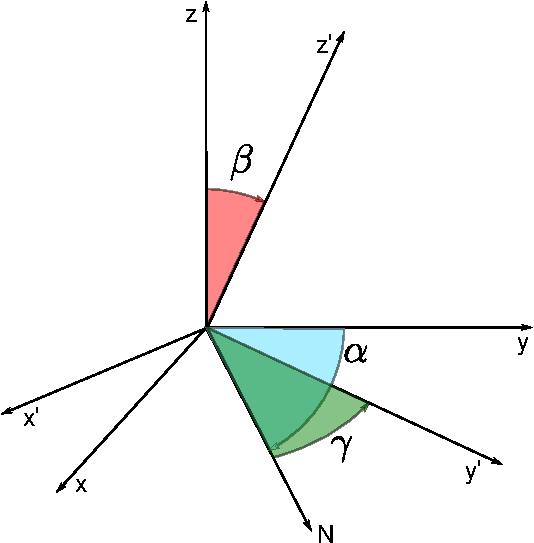
\includegraphics[width = 0.5\textwidth]{figs/eulerAnglesDefinition.pdf}
  \caption{Definition of the Euler angles $\alpha,\beta$ and $\gamma$ used to transform from the coordinate
           frame spanned by $x,y,z$ to the frame spanned by $x^\prime,y^\prime,z^\prime$. The intersection
           between $xy$- and $x^\prime y^\prime $-plane is denoted by $N$. Note that the sign of all angles
           are defined via the plane they are located in ($xy$- or $zy$-plane).}
  \label{fig:EulerAnglesDefinition}
\end{figure}

Molecular orbitals are expressed in terms of so-called real-spherical harmonics $S_{lm}$ (angular momentum $l$
and orientation $m$) which are linear combinations of their complex counter parts $Y_{lm}$, the eigenfunctions
of the angular momentum operator in $z$ direction $\hat{l}_z$. Since the $Y_{lm}$ are degenerate in $m$ for a
radial symmetric Hamiltonian, we are free to construct the linear combinations $S_{lm}$ without changing their
eigenvalue with respect to the Hamiltonian. Thus, the set of functions $S_{lm}$ may be constructed from the
functions $Y_{lm}$ and it may be shown that they represent a complete basis set for a given $l$\cite{Blanco1997}.

The rotation around the $z$-axis may be expressed in terms of the complex-spherical harmonics. In this basis
the rotation matrix associated to $\hat{R}_z$ is diagonal. Thus, the rotation around the $z$ axis may be
expressed in the basis of the real spherical harmonics as
\begin{align}
  \pmb{X}_l(\alpha) = \pmb{C}_l^\dagger \mathrm{Diag}(e^{im\alpha,m=-l,...l})\pmb{C}_l,
\end{align}
where $\mathrm{Diag}(e^{im\alpha,m=-l,...l})$ is the rotation matrix in basis of the complex-spherical harmonics,
and $\pmb{C}_l$ is the (unitary) transformation matrix between real and complex-spherical harmonics.

The matrix representation $\pmb{\Delta}_l(\alpha,\beta,\gamma)$ of the rotation of a set of functions expressed in
the basis of $S_{lm}$ by $\hat{R}$ is then given as
\begin{align}
  \pmb{\Delta}_l(\alpha,\beta,\gamma) = \pmb{X}_l(\alpha) \pmb{D}_l(\beta) \pmb{X}_l(\gamma).
  \label{eq:GeneralRotationWigner}
\end{align}
Here, $\pmb{D}_l(\beta)$ denotes the matrix of the rotation $\hat{R}_y(\beta)$ in the basis of $S_{lm}$
\cite{Blanco1997}.

In 2007 Pinchon and Hoggan\cite{Pinchon2007}, showed that $\pmb{D}_l(\beta)$ may be obtained by first exchanging the
coordinates of $y$ and $z$, rotating around $z$ and then exchanging the coordinates again. If we denote the matrix
for the exchange of $y$ and $z$ in the basis of $S_{lm}$ as $\pmb{J}_l$, we may write
\begin{align}
  \pmb{D}_l(\beta) = \pmb{J}_l \pmb{X}_l(\beta) \pmb{J}_l.
\end{align}
With this, Eq.~(\ref{eq:GeneralRotationWigner}) becomes
\begin{align}
  \pmb{\Delta}_l(\alpha,\beta,\gamma) = \pmb{X}_l(\alpha) \pmb{J}_l \pmb{X}_l(\beta) \pmb{J}_l \pmb{X}_l(\gamma).
  \label{eq:SphericalHarmonicsRotation}
\end{align}
In contrast to previous works\cite{Ivanic1996,Blanco1997}, only the exchange matrices
$\pmb{J}_l$ have to be calculated using recursive schemes, since an explicit expression for the matrix
$\pmb{X}_l(\alpha)$ is known.
It has only non-zero elements on its diagonal and anti-diagonal. For $l=2$, $\pmb{X}_2(\alpha)$ is given by
\begin{align}
  \pmb{X}_2(\alpha) = \begin{pmatrix}
                      \cos(2\alpha) & 0            & 0 & 0            & \sin(2\alpha) \\
                      0             & \cos(\alpha) & 0 & \sin(\alpha) & 0 \\
                      0             & 0            & 1 & 0            & 0 \\
                      0             & -\sin(\alpha)& 0 & \cos(\alpha) & 0 \\
                      -\sin(2\alpha)& 0            & 0 & 0            & \cos(2\alpha)
                      \end{pmatrix}.
\end{align}

The recurrence expressions for $\pmb{J}_l$ for $l \leq 1$ are given by
\begin{align}
  \begin{split}
    \pmb{G}^l_x \pmb{J}_l &= \pmb{J}_{l+1}\pmb{G}^l_x\\
    \pmb{G}^l_z \pmb{J}_l &= \pmb{J}_{l+1}\pmb{G}^l_y\\
    \pmb{G}^l_y \pmb{J}_l &= \pmb{J}_{l+1}\pmb{G}^l_z,
  \end{split}
  \label{eq:GauntTransformation}
\end{align}
where $\pmb{G}^l_x$, $\pmb{G}^l_y$ and $\pmb{G}^l_z$ are the matrices of the so-called Gaunt coefficients. Their
non-zero elements are given by
\begin{align}
  \begin{split}
    \kappa_l &= \frac{1}{2\sqrt{(2l+1)(2l+3)}},\\
    \left(\pmb{G}^l_x\right)_{2+k,k} = \left(\pmb{G}^l_x\right)_{2l+2-k,2l+2-k}&
    = \left(\pmb{G}^l_y\right)_{2l+2-k,k} = -\left(\pmb{G}^l_y\right)_{2+k,2l+2-k}\\
    &= \kappa_l\sqrt{k(k+1)},
    ~~~1\leq k \leq l-1,\\
    \left(\pmb{G}^l_x\right)_{k,k} = \left(\pmb{G}^l_x\right)_{2l+4-k,2l+2-k}
    &= \left(\pmb{G}^l_y\right)_{k,2l+2-k} = -\left(\pmb{G}^l_y\right)_{2l+4-k,k}\\
    &=-\kappa_l \sqrt{(2l+2-k)(2l+3-k},
    ~~~1\leq k \leq l,\\
    \left(\pmb{G}^l_x\right)_{l+2,l+2} = \left(\pmb{G}^l_y\right)_{l+2,l} &= \kappa_l \sqrt{2l(l+1)},\\
    \left(\pmb{G}^l_x\right)_{l+3,l+1} = \left(\pmb{G}^l_y\right)_{l+1,l+1} &= -\kappa_l \sqrt{2(l+1)(l+2)},\\
    \left(\pmb{G}^l_z\right)_{k+1,k} &= 2\kappa_l \sqrt{k(2l+2-k)},~~~ 1 \leq k \leq 2l+1.
  \end{split}
\end{align}
In order to calculate the entries of $\pmb{J}_l$, only the diagonal, non-zero block ($\hat{\pmb{G}}^l_z$)
of $\pmb{G}^l_z$ and $\pmb{G}^l_y$ are needed. $\pmb{J}_{l+1}$ may then be written as
\begin{align}
  \pmb{J}_{l+1} = \begin{pmatrix}
                    0      & ~ & 0 \\
                    \vdots &  \pmb{G}^l_y \pmb{J}_{l} \left(\hat{\pmb{G}}^l_z\right)^{-1} & \vdots\\
                    0      & ~ & 2^{-l}
                  \end{pmatrix},
  \label{eq:Recurrence}
\end{align}
where the central block of columns (all columns except the first and last one) are given by
$\pmb{G}^l_y \pmb{J}_{l} \left(\hat{\pmb{G}}^l_z\right)^{-1}$. The missing rows of the first and last column
can be constructed from the requirement of the matrix $\pmb{J}_{l}$ to be symmetric.

The matrices $\pmb{J}_{l}$ for $l=1$ and $l=0$ are given by
\begin{align}
  \pmb{J}_{0} = \begin{pmatrix}
                    1
                  \end{pmatrix},
\end{align}
and
\begin{align}
  \pmb{J}_{1} = \begin{pmatrix}
                  0 & -1 & 0 \\
                  -1&  0 & 0 \\
                  0 &  0 & 1
                \end{pmatrix}.
\end{align}
All other matrices for $l > 1$ may be computed using Eq.~(\ref{eq:Recurrence}).

\subsection{Copying and Pasting Molecular Orbitals}

Consider two molecules $A$ and $B$ which are identical up to translation and rotation. The molecular-orbitals set
$\{\psi^{A}_i\}$ of molecule $A$ is known and expressed in a set of spherical, atom-centered basis functions with
coefficients $\pmb{C}^A$. Our goal is to obtain the coefficients $\pmb{C}^B$ that correspond to the set
$\{\psi^{B}_i\}$ by translating and rotating the set $\{\psi^{A}_i\}$. Since the atoms of both molecules are the same,
their exists a one to one mapping of basis function shells. Thus, the translational part is trivially taken care of,
i.e. if the molecules are not rotated with respect to each other the coefficient matrices $\pmb{C}^A$ and
$\pmb{C}^B$ will be identical. In case of rotation, we first calculate the Euler angles ($\alpha_A$, $\beta_A$,
$\gamma_A$) for the rotation of the Cartesian frame to the internal frame of $A$. We can then rotate the
$\{\psi^{A}_i\}$ to the Cartesian frame by rotating the coefficient matrix in a shell-wise manner with the
transformation matrix $\pmb{\Delta}_l$ from Eq.~(\ref{eq:SphericalHarmonicsRotation}),
\begin{align}
  \left(\pmb{C}^\mathrm{Cart}\right)_{\mu_l} = \pmb{\Delta}_l(-\gamma_A,-\beta_A,-\alpha_A)\left(\pmb{C}^A\right)_{\mu_l},
\end{align}
where the subscript ${\mu_l}$ denotes the basis-function block associated to the shell $\mu_l$ with
angular momentum $l$.

The orbitals can then be rotated from the Cartesian frame to the internal frame of $B$ with the Euler angles
for the rotation of the Cartesian to the internal frame $B$ ($\alpha_B$, $\beta_B$, $\gamma_B$) as
\begin{align}
  \left(\pmb{C}^B\right)_{\mu_l} = \pmb{\Delta}_l(\alpha_B,\beta_B,\gamma_B)\left(\pmb{C}^\mathrm{Cart}\right)_{\mu_l}.
\end{align}

\subsection{Internal Frame Construction}

Each molecule is represented by the coordinates of its atoms $\{\pmb{a}_i\}$ in the Cartesian frame.
The internal $x$-axis $\pmb{e}_x$ is constructed as
\begin{align}
  \pmb{e}_x = \frac{(\pmb{a}_1-\pmb{a}_0)}{|\pmb{a}_1-\pmb{a}_0|},
\end{align}
the $y$-axis is constructed as
\begin{align}
  \pmb{e}_y = \frac{\pmb{t}_y}{|\pmb{t}_y|},
\end{align}
where $\pmb{t}_y$ is the orthogonalized difference vector between the coordinates of $1$ and $2$
which is defined with the difference vector $\pmb{d}_{21} = \pmb{a}_2-\pmb{a}_1$ as
\begin{align}
  \pmb{t}_y = \pmb{d}_{21}-\pmb{e}_x\pmb{e}_x^\dagger\pmb{d}_{21}.
\end{align}
The $z$-axis that belongs to a right-handed coordinate system can then be obtained as
\begin{align}
  \pmb{e}_z = \pmb{e}_x \times \pmb{e}_y.
\end{align}
Note that some special cases for highly symmetrical molecules need to be handled:
(i)   If the molecule consists of only one atom, the Cartesian frame is used as the internal frame.
(ii)  If the molecule consists of only two atoms, the vector $\pmb{d}_{21}$ is chosen to be the Cartesian
      $x$-axis if $\pmb{e}_x$ does not depend linearly on it. Otherwise the $y$-axis is chosen.
(iii) If the vector $\pmb{d}_{21}$ is linear depended on $\pmb{e}_x$, the difference vector $\pmb{d}_{31}$ is
      chosen for the construction of $\pmb{e}_y$. This is repeated until $\pmb{e}_y$ can be constructed. If there
      is no linear independent difference vector, the approach given in (ii) is used.

\section{Molecular Cavity and Surface Construction\label{sec:MolcSurface}}
This chapter describes the implementation of the molecular surface and cavity construction as
proposed by B. Delley\cite{Delley2006}.

\subsection{Molecular Surface Model}
Delley used for the molecular surface the zero-isosurface of a ball-and-stick-like
model function $F(\pmb{r})$ that varies continuously with the position $\pmb{r}_i$
and radii $R_i$ of the atoms. $F(\pmb{r})$ is given by
\begin{align}
  F(\pmb{r}) = 1+\sum_i f\left(\frac{(\pmb{r}-\pmb{r}_i)^2-R_i^2}{2R_sR_i} \right)
                +\sum_{i\neq j} f\left( \frac{\left[\pmb{r}-\pmb{r}_z(ij)\right]^2-R_z^2(ij)}{2R_s \max(R_z, 1.0~\text{au})} \right),
  \label{eq:delleyModelFunction}
\end{align}
where the auxiliary function $f(x)$ is given by
\begin{align}
  f(x) = -\exp(-\alpha x) + ax + b x^2.
\end{align}
The parameters $a$ and $b$ are obtained from the boundary conditions
$f(4/\alpha) = 0$ and $f^\prime(4/\alpha) = 0$. The radius of the solvent
probe is given by $R_s$. The parameter $R_z(ij)$ is the radius of a cylinder
that touches the spheres $i$ and $j$ as well as the solvent probe with radius
$R_s$, which in turn touches both spheres $i$ and $j$. It is given
with $S_i = R_i + R_s$ and $d_{ij} = |\pmb{r}_i-\pmb{r}_j|$ by
\begin{align}
  R_z(ij) = \sqrt{S_i^2 - \left( \frac{S_i^2+d_{ij}^2-S_j^2}{2d_{ij}} \right)^2}-R_s.
\end{align}
The parameter $\pmb{r}_z(ij)$ is the point of the orthogonal projection of the
point $\pmb{r}$ onto the bond between the spheres $i$ and $j$. If this projection
does not lie between spheres $i$ and $j$, $\pmb{r}_z(ij)$ is defined as the respective
bond end $\pmb{r}_i$ or $\pmb{r}_j$.
The bond part of the model (third term in Eq.~[\ref{eq:delleyModelFunction})] is restricted
to pairs $ij$ for which $d_{ij} \leq S_i+S_j$.


The model function $F(\pmb{r})$ can be understood as placing a function
$1-\exp\left[-\alpha (r-R)\right]$ on every atom and on every bond of the molecule.
Thus, $F(\pmb{r})$ will have large negative values within the molecule, a value of
$0$ at the molecular surface and a value of $1$ far outside the molecule. The parameter
$\alpha$ controls how sharp the superposition of functions from different spheres or
cylinders is. It is typically set to $\alpha = 50.0$. For small values of $\alpha$ the
surface may become blurred.

\subsection{Molecular Surface Discretization}
For the application of continuum solvation models\cite{Tomasi2005} it is necessary to
discretize the surface into small areas with one representative point each, so-called tesserae.
This is achieved by atom-wise projection of spherical integration grids to the molecular
surface as shown in Fig.~\ref{fig:delleySurfaceConstruction}(a). The normal vectors $\pmb{n}_p$
at the position of the grid point $\pmb{r}_p$, which are needed for some continuum models, are obtained as
normalized vectors with the direction of $\left.\nabla F(\pmb{r})\right|_{\pmb{r}=\pmb{r}_p}$.
In \textsc{Serenity} the standard spherical grid point distributions by Lebedev and Laikov are used.
\begin{figure}
	\centering
	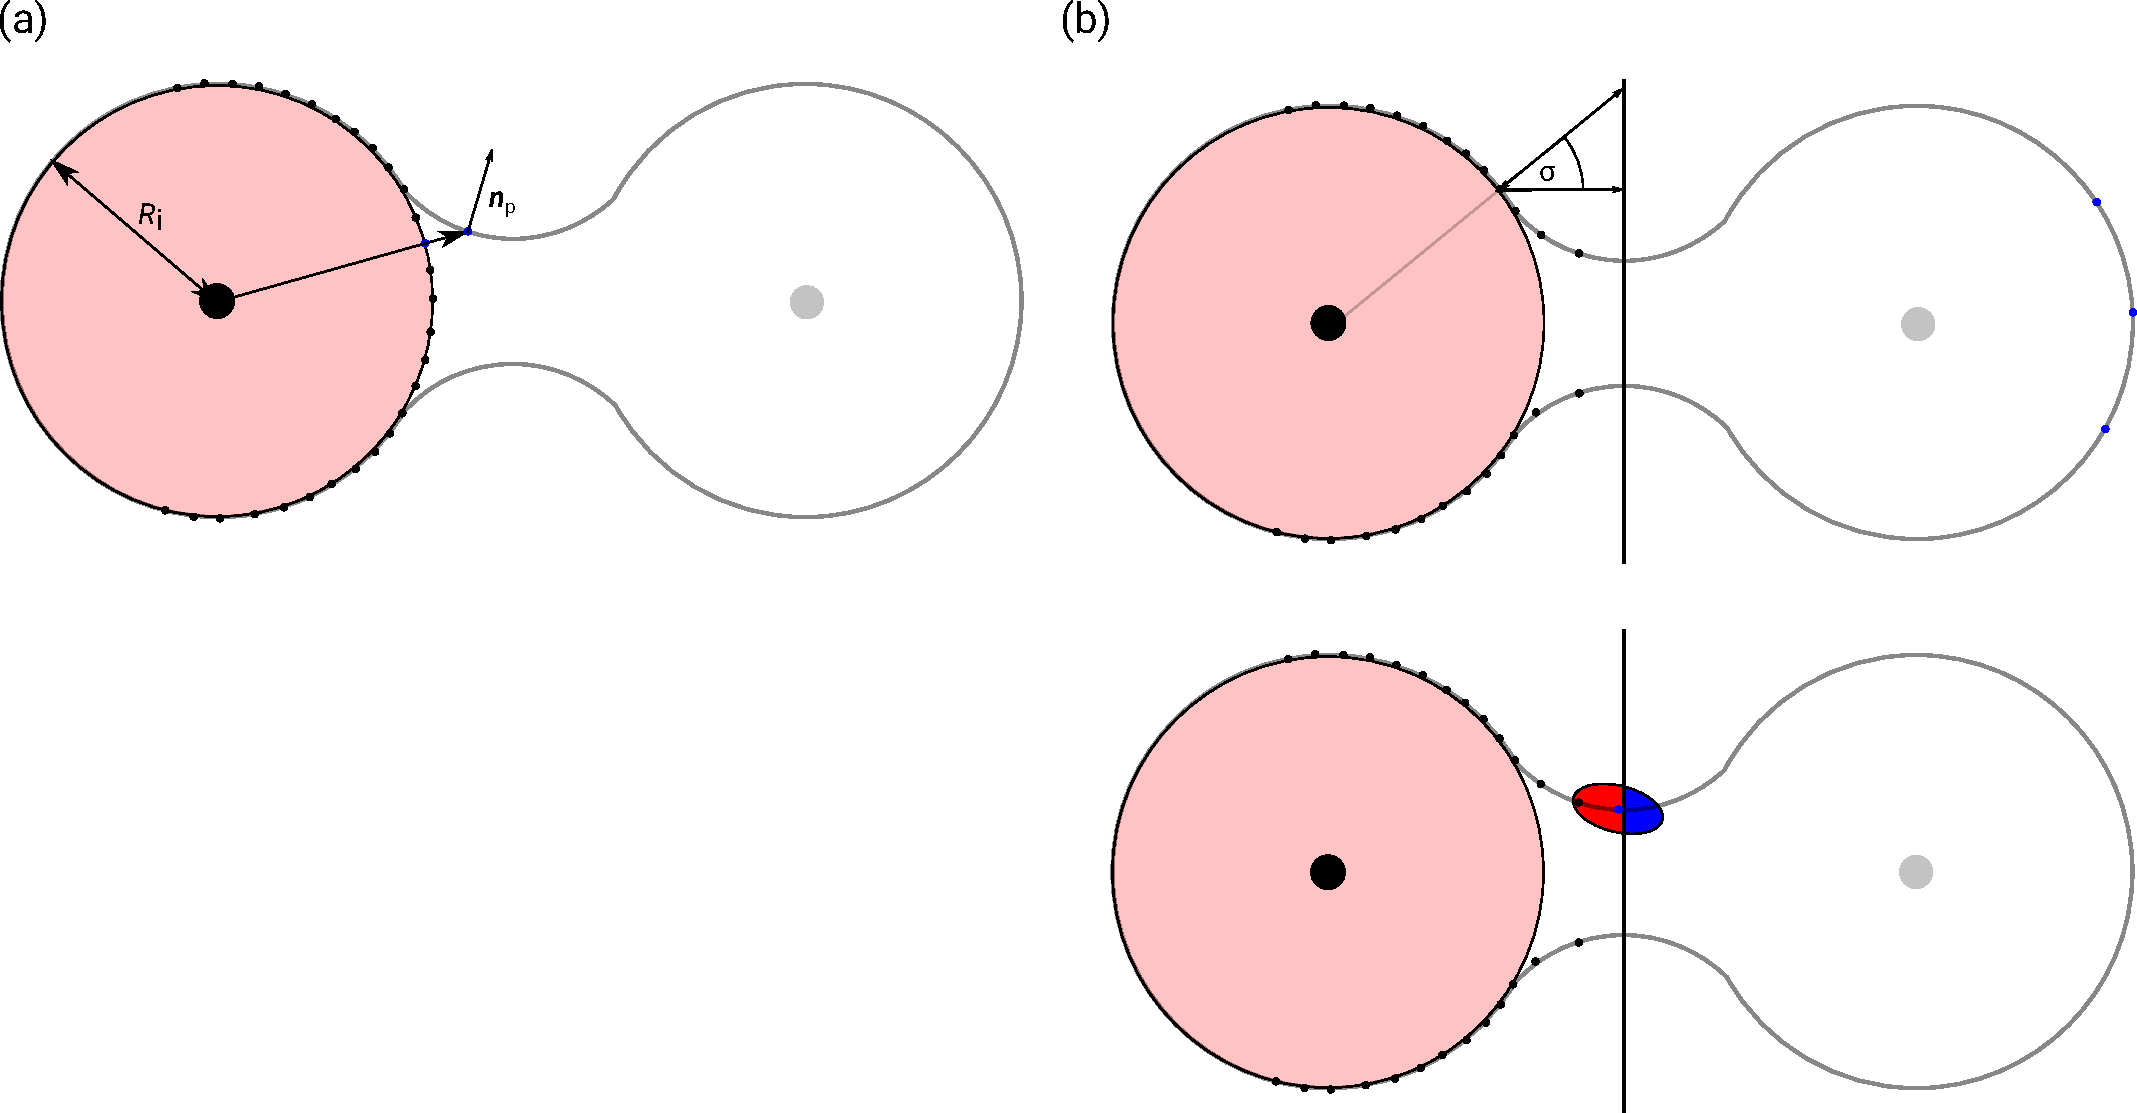
\includegraphics[width=0.95\textwidth]{figs/delleyFigure.pdf}
	\caption{Schematic of the surface mesh construction for a diatomic molecule.
			 (a) Projection of the spherical grid points to the molecular surface, and
			     construction of the normal vector $\pmb{n}_p$.
			 (b) Area scaling and cutting for grid points on the bond part of the molecular
			     surface.}
	\label{fig:delleySurfaceConstruction}
\end{figure}

The initial weights or areas $A_p^\prime$ associated to each point are calculated as
\begin{align}
	A_p^\prime = 4.0\pi A_{i,p}^{u}|\pmb{r}_p-\pmb{r}_i|^2,
\end{align}
where $A_{i,p}^{u}$ is the weight of the grid point on the unit sphere surrounding sphere $i$.
These weights are then scaled by the skew projection on the bond plane as $A_p^s = \sin(\sigma) A_p^\prime$
(see Fig.~\ref{fig:delleySurfaceConstruction}(b)) if they fall on the bond part of the surface
($\pmb{r}_z(ij) \neq \pmb{r}_i$ and $\pmb{r}_z(ij) \neq \pmb{r}_j$) and a bond between the spheres exists.
We then define planes $P(ij)$ orthogonal to each bond $ij$ (plane normal vectors
$\pmb{n}_\mathrm{bond} = \frac{\pmb{r}_i-\pmb{r}_j}{|\pmb{r}_i-\pmb{r}_j|}$) which contain the points
$\pmb{c}_\mathrm{bond} = \frac{R_i}{R_i+R_j} \pmb{r}_i +\frac{R_j}{R_i+R_j} \pmb{r}_j$, which
are the weighted centers of the bonds. We then consider each point on a bond to be an ellipse with
radial vectors $\pmb{r}_1$ and $\pmb{r}_2$ ($\pmb{r}_1^\dagger\pmb{r}_2 = 0$) given as
\begin{align}
	\pmb{r} = \pmb{r}_1 \cos(t) + \pmb{r}_2 \sin(t),~t\in [0,2\pi].
\end{align}

The ellipse construction is illustrated in Fig.~\ref{fig:ellipseConstruction}.
The direction of $\pmb{r}_1$ is obtained as the direction $\pmb{d}_s$ of the intersection between
the plane on the original sphere (its normal vector is equal to the vector $\pmb{n}_\mathrm{pro}$
used for the projection of the point to the surface) and the plane containing
the projected point, described by the normal vector $\pmb{n}_p$. The direction of $\pmb{r}_2$ is obtained by
requiring that $\pmb{r}_2$ is orthogonal to $\pmb{r}_1$ and $\pmb{n}_p$.

The length of the radial vectors is calculated by projecting a point on the circle
on the initial sphere to the plane on the molecular surface as shown in Fig.~\ref{fig:ellipseConstruction}
for $\pmb{r}_1$. The same procedure is applied for $\pmb{r}_2$. The vectors are then scaled such that
the ellipse contains the area $A_p^s$.


\begin{figure}[H]
	\centering
	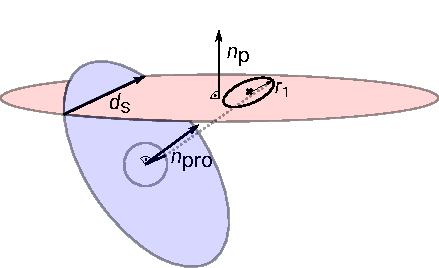
\includegraphics[width=0.8\textwidth]{figs/ellipseConstruction.pdf}
	\caption{Illustration of the ellipse construction for the area scaling.
	         The direction of the intersection between the plane on the initial sphere ($blue$)
	         and the plane on the molecular surface $red$ is denoted with $\pmb{d}_s$.
	         The vector $\pmb{r}_1$ is obtained by going from the center of the circle on the
	         initial sphere in direction of $\pmb{d}_s$ according to the area of the circle.
	         Then a line is constructed containing this point with direction $\pmb{n}_\mathrm{pro}$,
	         and the intersection with the $red$ plane is calculated. The same is done for $\pmb{r}_2$.
	         Both vectors are then scaled such that the ellipse has the desired area.}
	\label{fig:ellipseConstruction}
\end{figure}

If an ellipse is cut by a plane $P(ij)$ [see Fig.~\ref{fig:delleySurfaceConstruction}(b)], the area and the center
of gravity $\pmb{r}_{p,\mathrm{grav}}$ not hidden by the plane from the perspective of the owning atom is calculated.
If the ellipse is completely hidden by the plane, the point is dropped.
The center of gravity is projected back to the molecular surface along the direction
$\pmb{r}_{p,\mathrm{grav}}-\pmb{r}_i$ and a new ellipse is constructed. This procedure is repeated for all $j$ bonding
with $i$. This construction ensures that all points remain on the bond side of their initial atoms.

\section{Cholesky Decomposition}

The Cholesky decomposition is a mathematical procedure that enables to speed up many applications in theoretical chemistry. It allows to decompose a hermitian, positive (semi-)definite matrix $M$ into a lower triangular matrix $L$ and its transposed

\begin{equation}
M=LL^T.
\end{equation}

It can for example be applied to decompose the two-electron four-center integral matrix  into three index objects

\begin{equation}\label{CDMatrix}
\langle \mu \nu | \lambda \sigma \rangle = \sum_P^M \langle \mu \nu | P \rangle \langle P | \lambda \sigma \rangle = \sum_P^M L^P_{\mu\nu} L^P_{\lambda\sigma} ,
\end{equation}

where the greek letters are indices of the basis functions $\phi_\mu$ and the counting index $P$ refers to which Cholesky vector is used. This Cholesky vector is equivalent to the $P$th column in the matrix $L$. Consequently, $M$ is the number of Columns in $L$ or the number of Cholesky vectors. The mapping of the column or row indices of the original matrix to the indices of the Choleky vectors is called the Cholesky basis.\\

To see why this decomposition is useful in speeding up calculations, one can compare it to the well established resolution of the identity (RI) approach. Here, the basis is projected to the space of a prefitted auxiliary basis so that it seems that the identity of the auxiliary basis was inserted into the original expression
\begin{equation}\label{RIFull}
\langle \mu \nu | \lambda \sigma \rangle \approx \sum_{P,Q} \langle \mu \nu | P \rangle \langle P | Q \rangle^{-1} \langle Q | \lambda \sigma \rangle .
\end{equation} 

If simplified using

\begin{equation}
B_{\mu \nu,Q} = \sum_{P} \langle \mu \nu | P \rangle \langle P | Q \rangle^{-1/2},
\end{equation}

the equation becomes 

\begin{equation}
\langle \mu \nu | \lambda \sigma \rangle \approx \sum_{Q} B_{\mu \nu,Q} B_{\lambda \sigma,Q}.
\end{equation} 

Comparing this result to Eq.~\ref{CDMatrix} it becomes evident that they are equivalent and can be evaluated with similar efficiency. However, one has to keep in mind that, in general, the basis obtained in all Cholesky procedures is larger than the prefitted auxiliary basis sets used in the RI approach. As a result, Cholesky based calculations will always be slower than comparable RI calculations if available.\\

The advantage of Cholesky Decomposition compared to RI is that, as shown in the following sections, it offers error control for all elements in the matrix that is decomposed. This is in contrast to the RI approach, where the auxiliary basis is fitted to reproduce on particular metric (like for example the Coulomb energy contribution), but a reconstruction of the original matrix as in Eq.~\ref{RIFull} will contain significant errors.


\subsection{The Decomposition Algorithm}

A basic algorithm to perform the Cholesky decomposition is given below (Algorithm 1). It features pivoting, which means that no full decomposition is performed but that the decomposition is stopped once a certain accuracy in each matrix element (given by the decomposition threshold $\delta$ ) is reached. The drawback of this algorithm is that it requires the original matrix $M$ to be stored in memory in its entirety. This normally is no problem but the full two-electron four-center integrals can quickly take up more memory than available in modern clusters.

\begin{figure}[h!]
	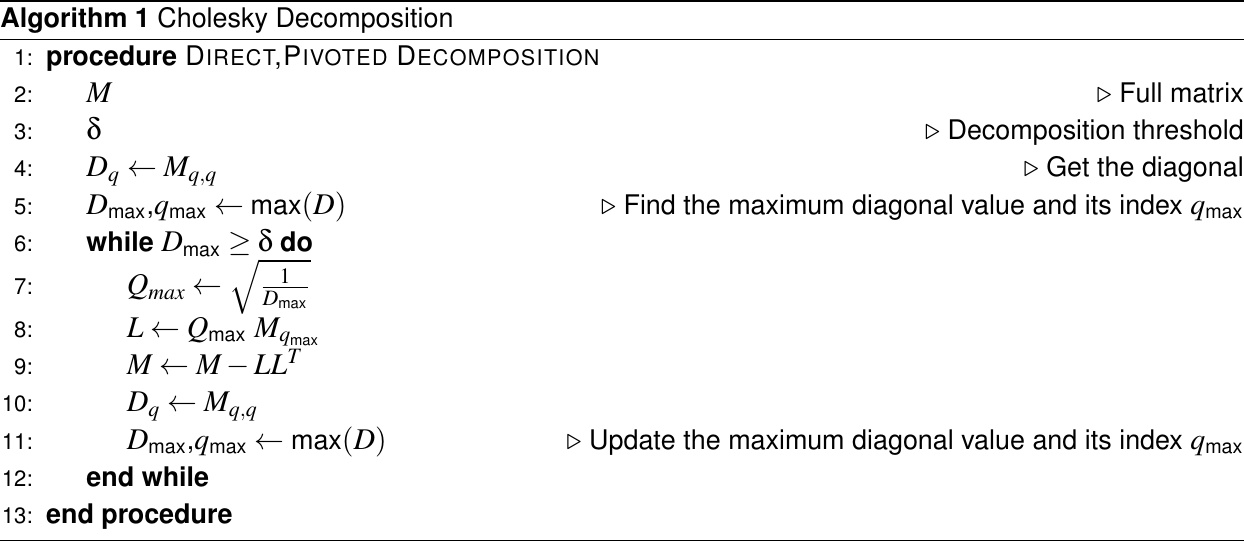
\includegraphics[width=\textwidth]{cholesky/algorithm1.png}
\end{figure}

To circumvent this problem, a memory efficient algorithm is implemented in \textsc{Serenity} (Algorithm 2). This algorithm firstly analyzes the diagonal to find the columns that have the potential to contribute to the Cholesky vectors and summarizes the corresponding indices in the reduced set $\mathcal{R}$. Then, the most significant elements in $\mathcal{R}$ are determined and summarized in the qualified set $\mathcal{Q}$. In general, this set is obtained by checking if the diagonal element is larger than $D_\text{min}$ but, in practice, the size of $\mathcal{Q}$ is also limited to a smaller number of elements to ensure memory and general efficiency (this avoids the calculation and later subtraction of too many elements that ultimately do not contribute to the Cholesky vectors, due to linear dependencies in $\mathcal{Q}$). As a result, in each iteration only the subset of integrals spanned by $\mathcal{Q}$ and $\mathcal{R}$ has to be calculated. Furthermore, the quite expensive subtraction step only has to be performed on that subset of integrals during each iteration. This also means that, in the end, the Choleksy vectors are calculated only in the subspace of $\mathcal{R}$ and have to be mapped to the corresponding indices in the complete set $\mathcal{S}$. Another important feature of this algorithm is checking for numerical errors. These can lead to small negative entries in the diagonal, which in turn can lead to errors in the calculation of $Q_{\text{max}}$. The last feature worth mentioning is the pre-screening of the qualified set $\mathcal{Q}$ for all elements that will actually contribute to the Cholesky vectors. This step exploits the fact that a decomposition of a matrix spanned by $\mathcal{Q}$ and $\mathcal{R}$ will yield the same contributing indices as the decomposition of the matrix spanned by $\mathcal{Q}$ and $\mathcal{Q}$. Since the dimension of $\mathcal{Q}$ is significantly lower than that of $\mathcal{R}$, the overhead created by additional decomposition step is negligible compared to the computational savings in the following steps.

\begin{figure}
	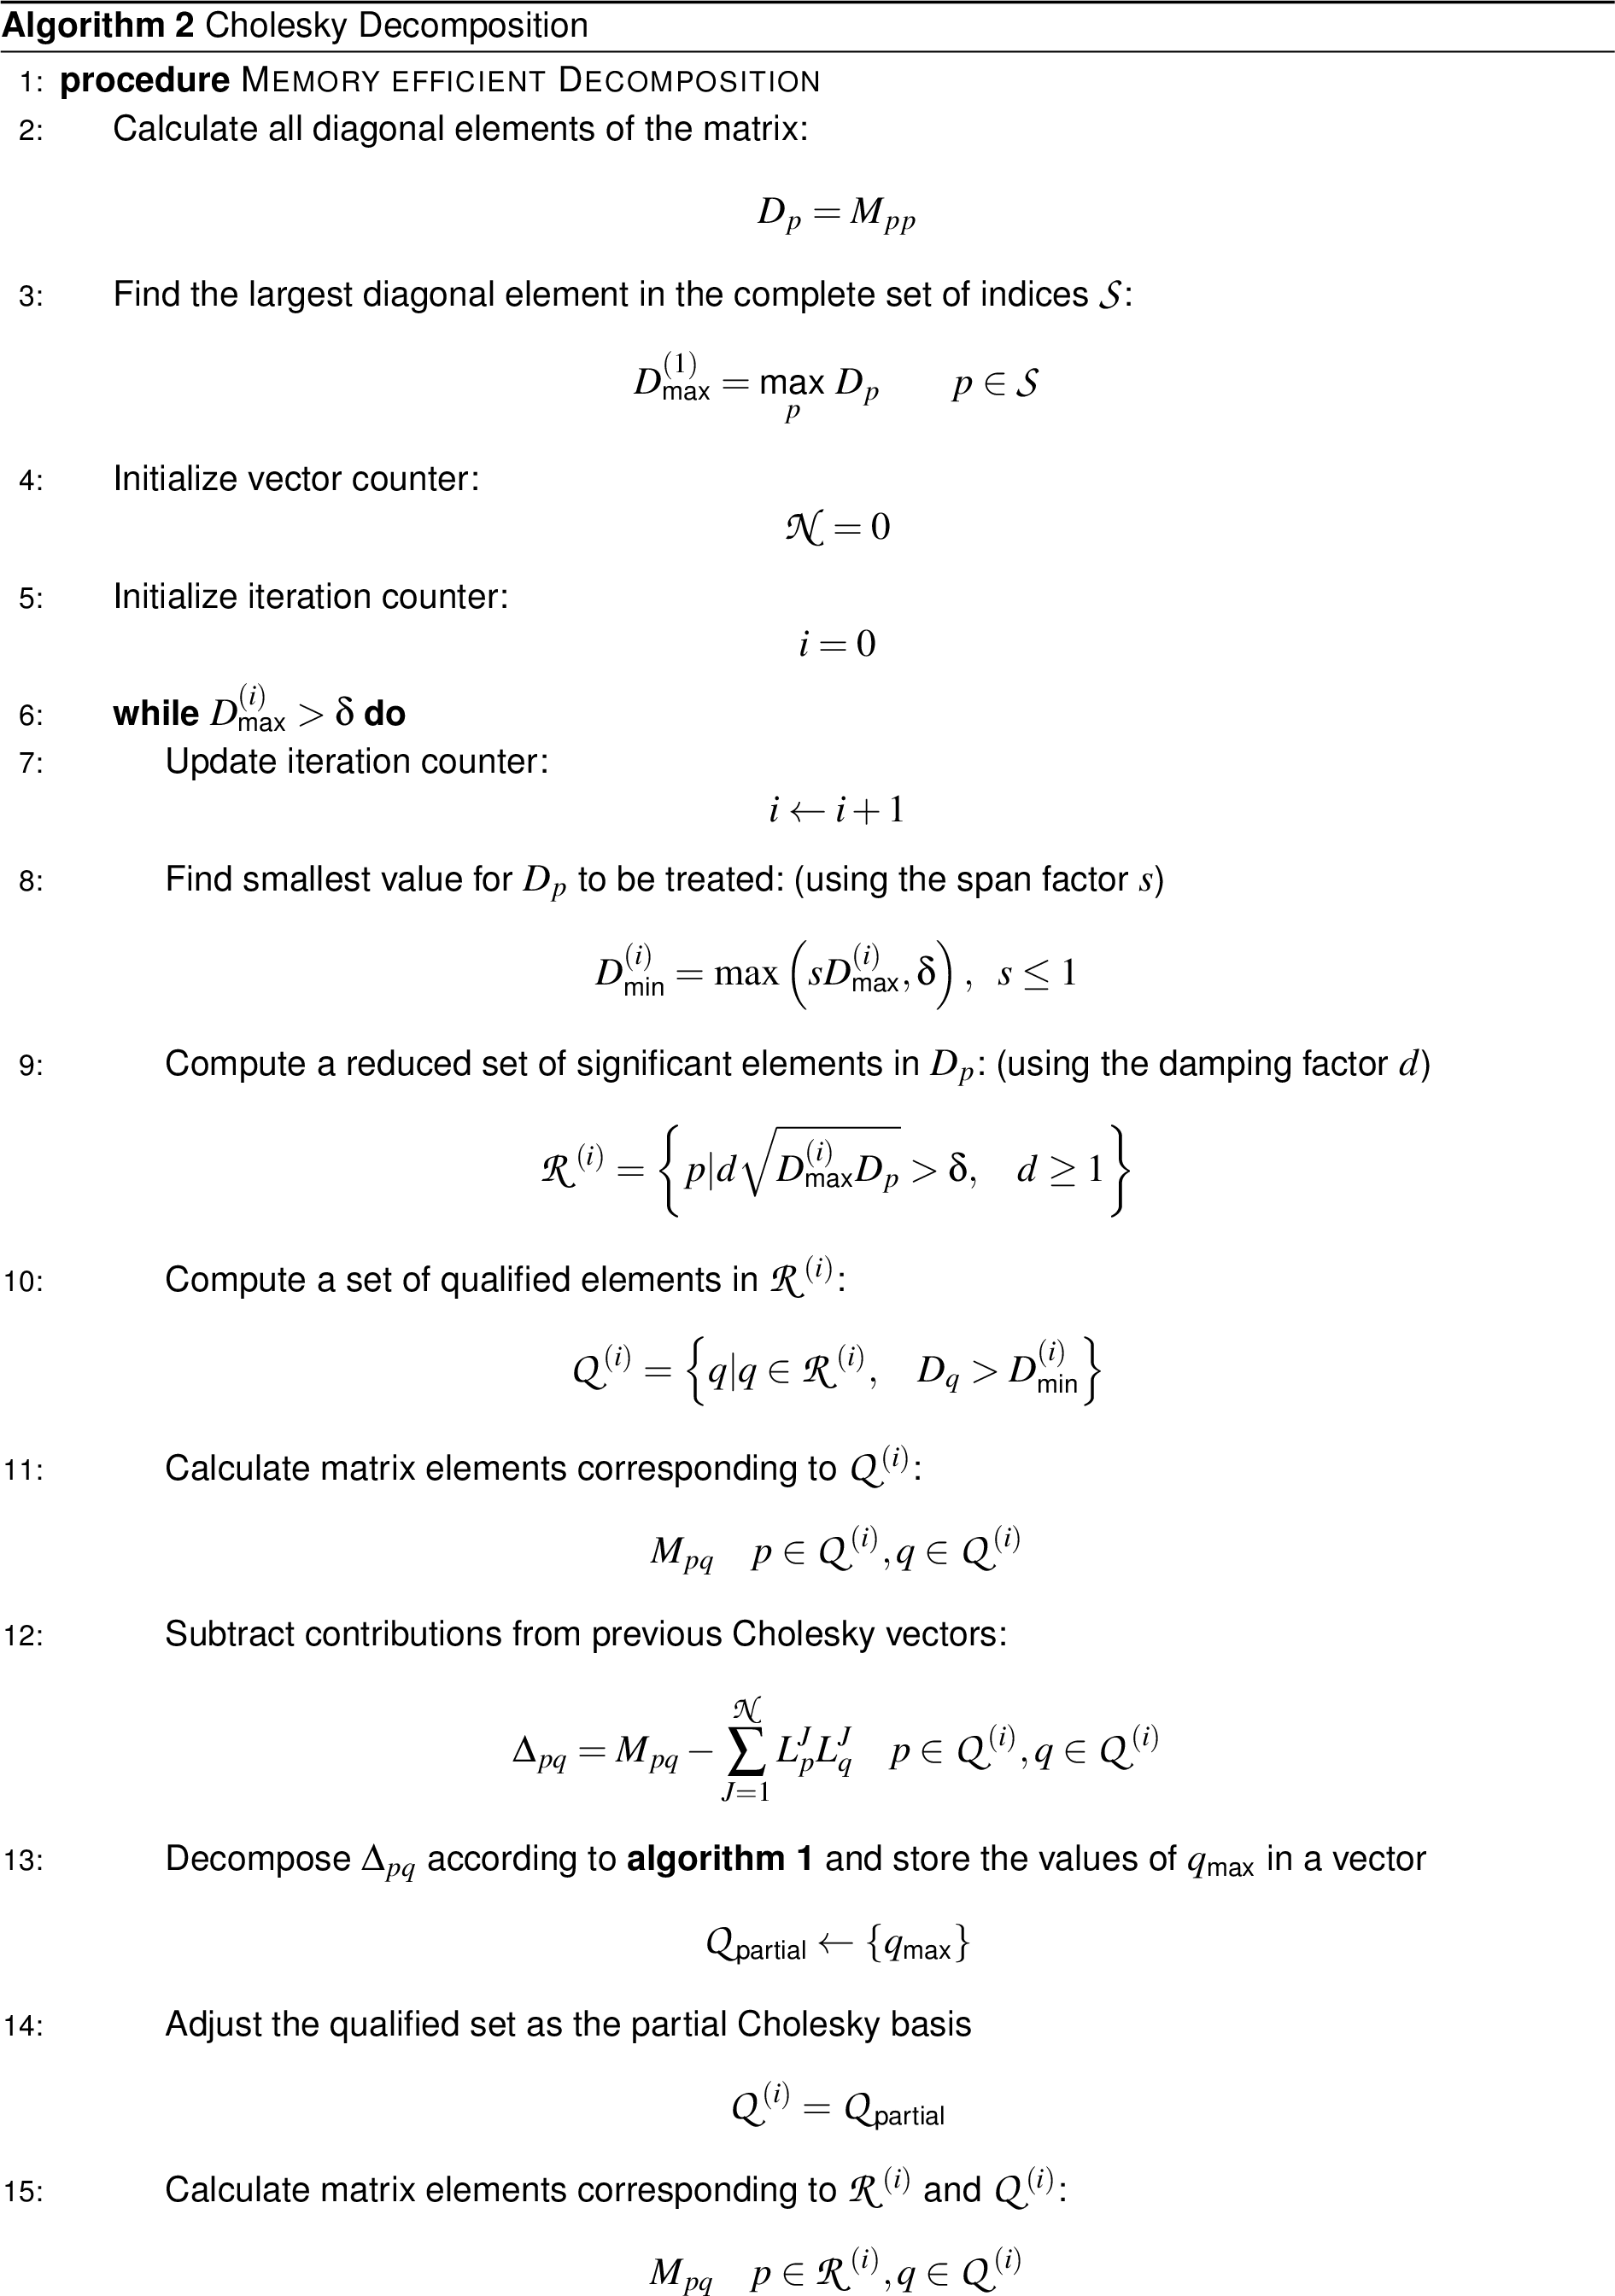
\includegraphics[width=\textwidth]{cholesky/algorithm2_1.png}
\end{figure}

\begin{figure}
	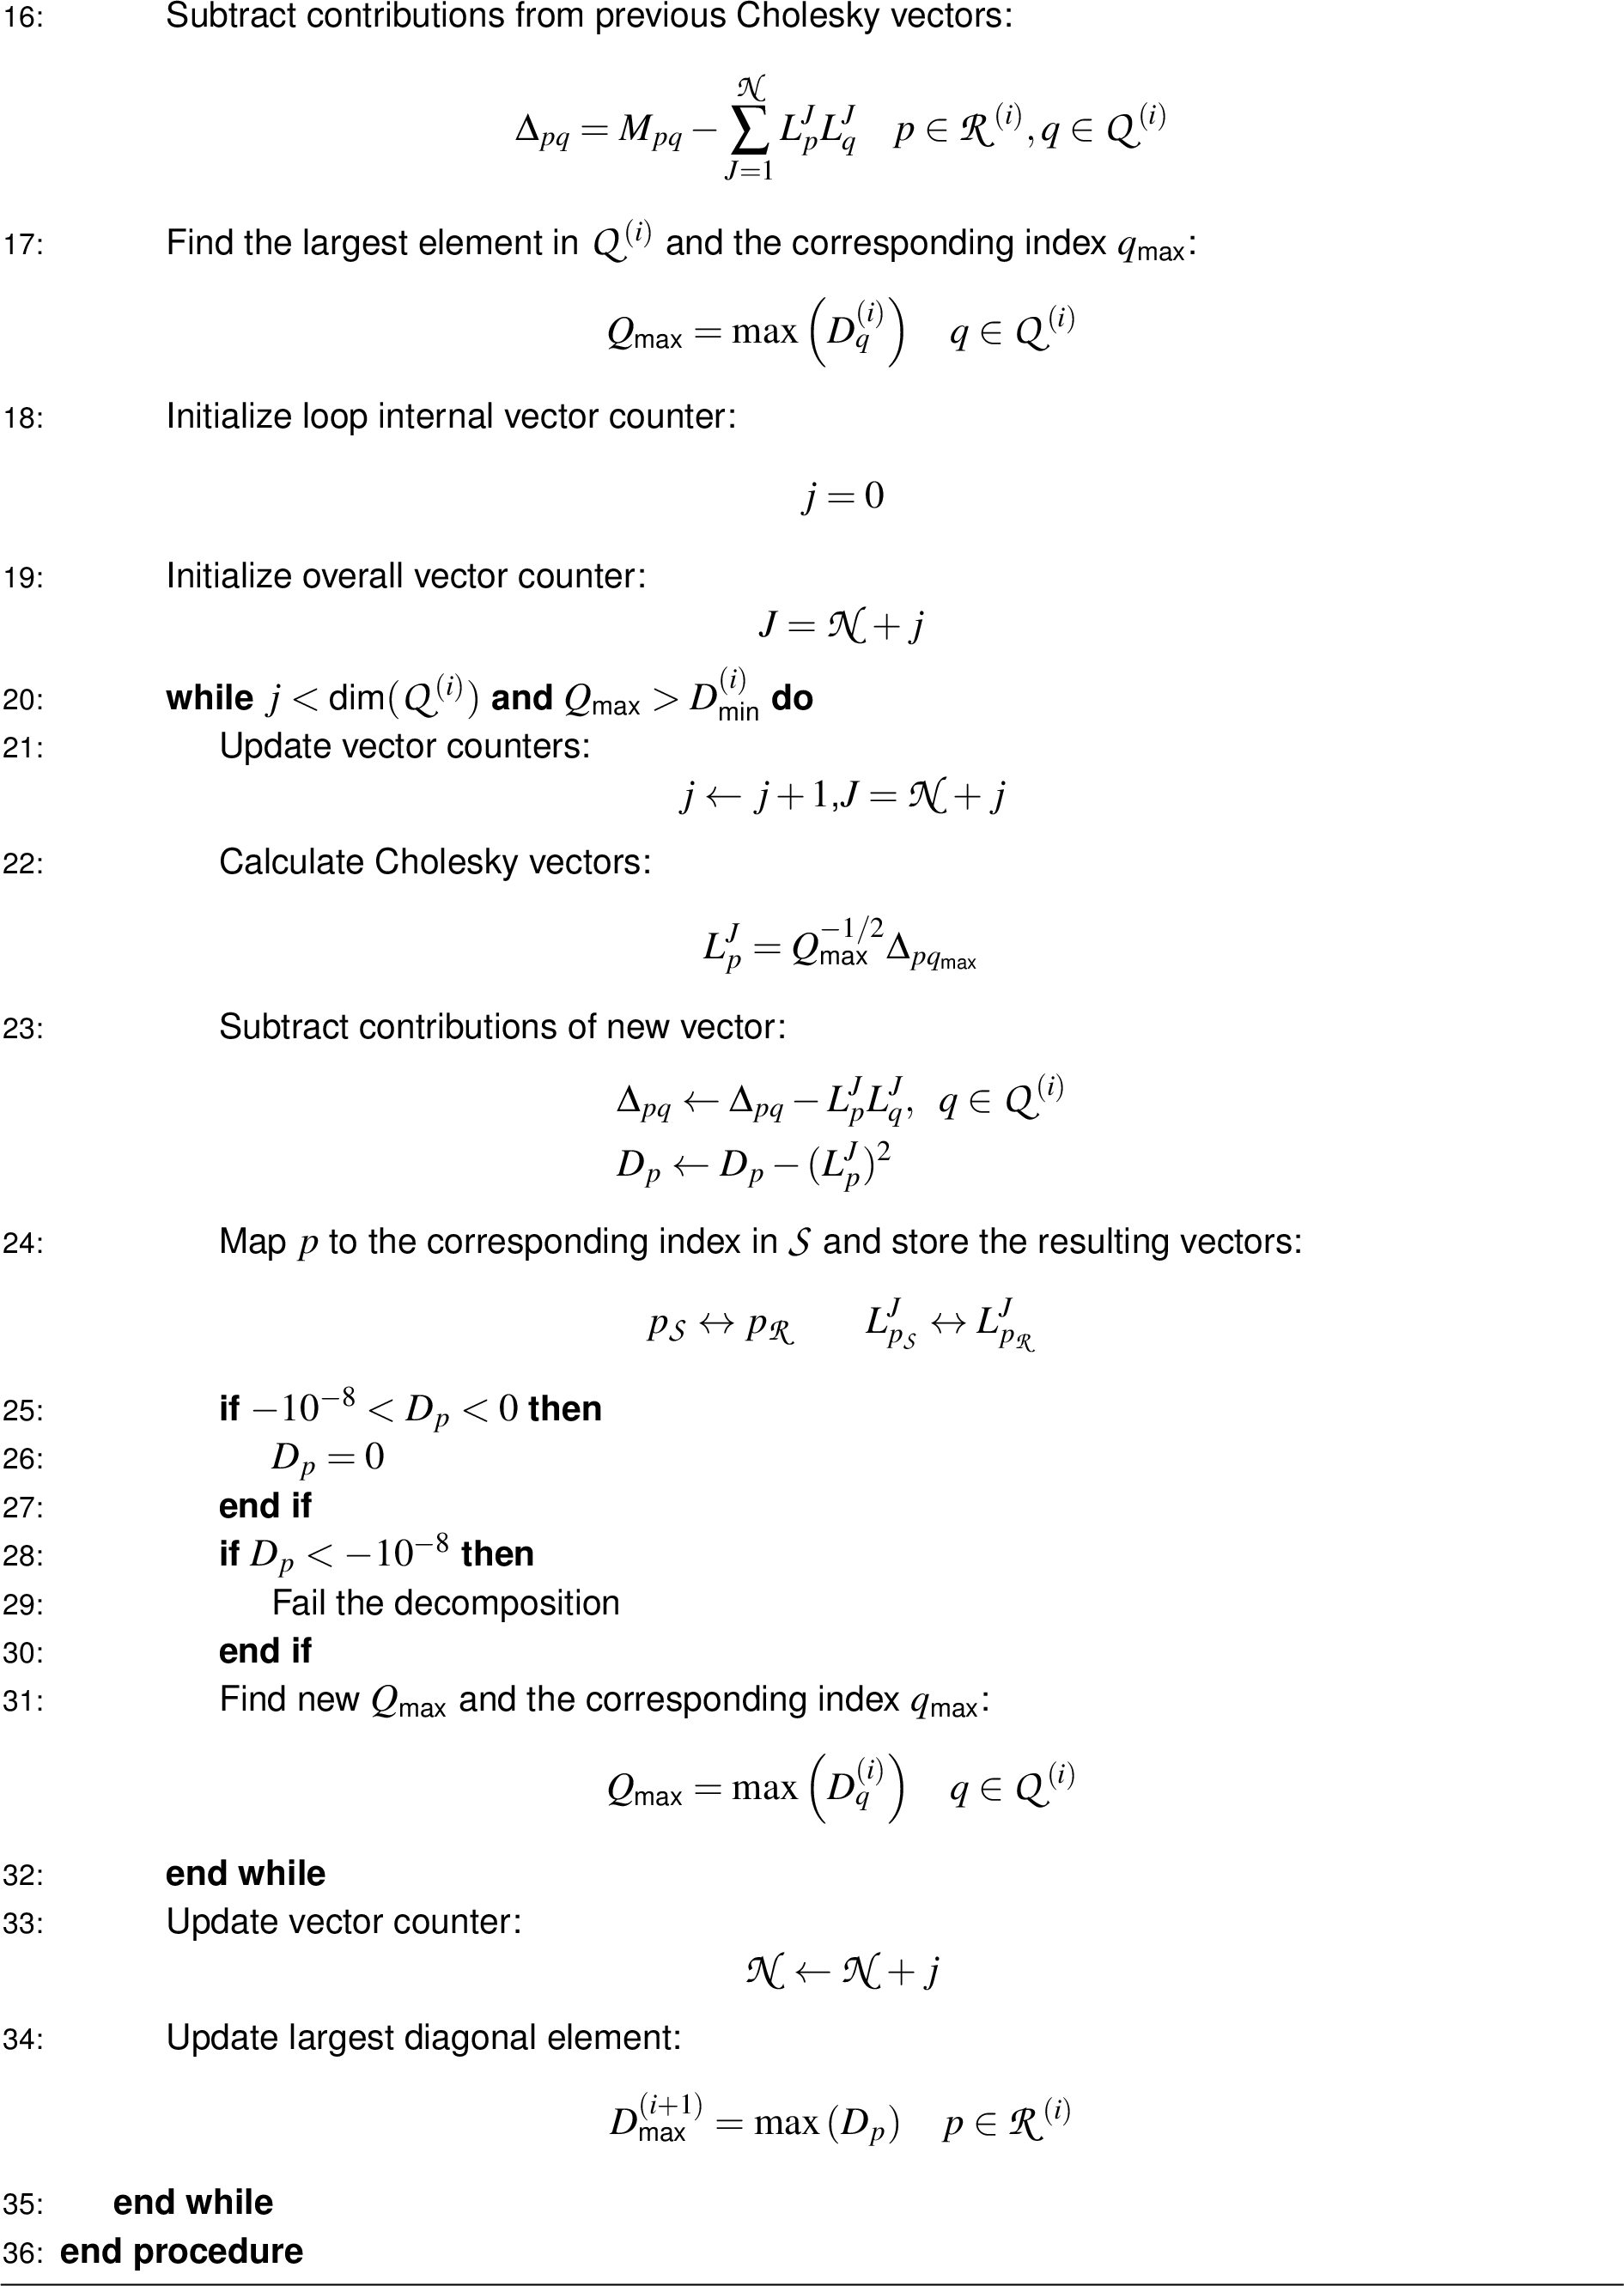
\includegraphics[width=\textwidth]{cholesky/algorithm2_2.png}
\end{figure}



\subsection{The Atomic Cholesky Decomposition}

One major problem of the generic Cholesky decomposition approach is that it needs to decompose the complete two-electron four-center integral matrix. This is easily feasible for small systems, but at the latest when it is no longer possible to hold the full matrix in memory it becomes a time-determining step. In order to remove this unfavorable behavior, an additional approximation can be introduced. Instead of enforcing a strict error control in all integrals, the atomic Cholesky decomposition (ACD) only enforces this strict control in the integrals where all four basis functions are centered at the same point. This is done by decomposing the two-electron four-center integrals of the isolated atom types
\begin{equation}\label{ACDMAtrix}
\langle \mu \nu | \lambda \sigma \rangle \approx \sum_P^M L^P_{\mu\nu} L^P_{\lambda \sigma} ,
\end{equation}
where $P$ is spans the subspace of all linearly independent basis function products $\phi_\mu \phi_\nu$. This identification allows to generate a new auxiliary basis set, where the basis functions are chosen as $$\phi_P = \phi_\mu \phi_\nu .$$ 
As a result, if we use the obtained auxiliary ACD basis in a way similar to the RI approach
\begin{equation}\label{ACDFormalism}
\langle \mu \nu | \lambda \sigma \rangle \approx \sum_{P,Q} \langle \mu \nu | P \rangle \langle P | Q \rangle^{-1} \langle Q | \lambda \sigma \rangle ,
\end{equation} 
one still retains strict error control for the integrals centered only at one atom. For all other elements residing on more than one center an error minimization is retained. The big advantage of this method is that the generation of the auxiliary basis set does not scale with the size of the system itself but only with the number of different atom types and the size of the basis set used, enabling it to generate these auxiliary basis sets on the fly for each calculation with minimal overhead.

\subsection{The Atomic Compact Cholesky Basis}

The big problem inherent to the ACD approach are the basis-function products used as the new basis functions, as these are contracted Gaussian-type functions 
\begin{equation}
\phi_\mu^c = \sum_i^{n_i} c_i \phi_{i,\mu}^p 
\end{equation}
and their products are given as
\begin{equation}
\phi_P = \phi_\mu^c \phi_\nu^c = \sum_i^{n_i} \sum_j^{n_j} c_i c_j \phi_{i,\mu}^p \phi_{j,\nu}^p .
\end{equation}
It can be easily seen that the number of primitive basis functions for one contracted basis function scales with $\mathcal{O}(n_i^2)$, which makes the computation of the integrals very expensive or even impossible with the corresponding libraries used in \textit{Serenity}. 
The atomic compact Cholesky decomposition (ACCD) makes use of the fact that linear dependencies within this massive space of primitive basis functions will occur again. They can be removed by setting up the two-electron two-center integral matrix of the primitive basis functions in one contracted basis function, and decompose it as
\begin{equation}
\langle	\mu^p | \nu^p \rangle \approx \sum_P^M L^P_{\mu^p} L^P_{\nu^p} ,
\end{equation}
allowing to remove primitive basis functions from the basis, which can be represented by linear combinations of other primitive basis functions. In practice, this procedure drastically reduces the number of primitive basis functions and makes the A(C)CD approach feasible for all systems at the cost of the additional approximation introduced in the decomposition and the corresponding reduction in the accuracy of the integrals.


\subsection{Generating Integrals Equivalent to Cholesky Vectors}

The basis sets generated with the ACD and ACCD approach can directly be used in an existing RI framework in place of the conventional RI auxiliary basis sets. As this approach directly fits the integrals needed and not any other metric, the A(C)CD auxiliary basis sets can be used in place of all types of RI auxiliary basis sets (RI-J, RI-K, RI-C,...). Moreover, these basis sets can be used to generate pseudo Cholesky vectors as
\begin{equation}
B^Q_{\mu \nu} = \sum_{P} \langle \mu \nu | P \rangle \langle P | Q \rangle^{-1/2} ,
\end{equation}
which can be used similar to Cholesky vectors to reconstruct the full two-electron four-center integral matrix
\begin{equation}
\langle \mu \nu | \lambda \sigma \rangle \approx \sum_{Q} B^Q_{\mu \nu} B^Q_{\lambda \sigma}.
\end{equation} 
Therefore, the intermediates $B^Q_{\mu \nu}$ can be used in place of the full Cholesky vectors $L^Q_{\mu \nu}$ and in the corresponding algorithms.

\subsection{Hartree--Fock Using Full Cholesky Vectors}

The big advantage of all density fitting procedures is that the number of integrals that have to be computed can be reduced drastically. This, however, comes with the drawback that you have to perform more computational steps to obtain the final contributions to the metric you are calculating. \textit{E.g.}, in order to calculate the Coulomb contribution to the Fock matrix, one can rewrite the expression in terms of the Cholesky vectors as
\begin{equation}
F^{Coul}_{\lambda\sigma} = \sum_{\mu\nu}^{N} P_{\mu\nu} \langle \mu \nu | \lambda \sigma \rangle = \sum_{\mu\nu}^{N} P_{\mu\nu} \sum_{J}^{M} L^J_{\lambda\sigma} L^J_{\mu\nu} .
\end{equation}
It is evident that an evaluation in this manner would scale with $\mathcal{O}(MN^4)$ compared to the evaluation of the full integrals, which scales with $\mathcal{O}(N^4)$. By rewriting the equation above and splitting it into two steps, this unfavorable behavior can be circumvented:

\begin{equation}
V^J = \sum_{\mu\nu}^{N} P_{\mu\nu} L^J_{\mu\nu} ,
\end{equation}

\begin{equation}
F^{Coul}_{\lambda\sigma} =  \sum_{J}^{M} L^J_{\lambda\sigma} V^J  .
\end{equation}

This results in a formal scaling of $\mathcal{O}(2MN^2)$ as long as all integrals $L^J_{\mu \nu}$ can be held in memory. If that is not the case, the integrals either have to be written to disk and then be loaded again for the second step or they have to be calculated twice. For the exchange contribution, the expression can be rewritten in a similar fashion as

\begin{equation}
F^{Exc}_{\lambda\sigma} = -\frac{1}{2} \sum_{\mu\nu}^{N} P_{\mu\nu} \langle \mu \sigma | \lambda \nu \rangle = -\frac{1}{2} \sum_{\mu \nu}^{N} P_{\mu\nu} \sum_{J}^{M} L^J_{\mu\sigma}  L^J_{\lambda\nu} = -\frac{1}{2} \sum_{J}^{M} \sum_{\mu}^{N} L^J_{\mu\sigma} \sum_{\nu}^{N} P_{\mu\nu} L^J_{\lambda\nu} .
\end{equation}

If this equation is reordered and the density matrix is expressed as product of the orbital coefficients, one can obtain 
\begin{equation}
F^{Exc}_{\lambda\sigma} = -\sum_{J}^{M} \sum_i^{occ} \sum_{\mu}^{N} c_{\mu i} L^J_{\mu\sigma}  \sum_{\nu}^{N}  c_{\nu i}  L^J_{\lambda\nu} .
\end{equation}

At this point, one can again identify intermediates

\begin{equation}
L^J_{i \sigma} = \sum_\mu c_{\mu i} L^J_{\mu \sigma} ,
\end{equation}

and thereby evaluate the complete exchange contribution efficiently as

\begin{equation}
F^{Exc}_{\lambda\sigma} = -\sum_{J}^{M} \sum_i^{occ} L^J_{i \sigma} L^J_{i \lambda} .
\end{equation}

Problems in this formalism arise when intermediates $L^J_{i \sigma}$ cannot be stored in memory, which means that they have to be recalculated (multiple times) in each SCF iteration. \textbf{Note}: In case of the A(C)CD approach, the Cholesky vectors are obtained as 
\begin{equation}
L^J_{\mu \sigma} = \sum_{P} \langle \mu \sigma | P \rangle \langle P | J \rangle^{-1/2} ,
\end{equation}
making it difficult to write a memory-efficient implementation that does not involve the recalculation of integrals.



% ========================
%   Citation and License
% ========================

\clearpage
\input{misc/cite.tex}

\clearpage
\printbibliography

% ==============
%   Appendices
% ==============
\clearpage
\appendix

\input{examples/examples.tex}

\clearpage

\input{misc/history.tex}

\clearpage

\input{misc/lgpl.tex}
\end{document}